


\begin{document}

\noindent This report describes design, implementation and test of two voltage amplifiers. One consisting of negative metal oxide semconducting field effect transistors (NMOS). The other comprised of bipolar junction transistors. Figure \ref{fig:blockdiagram2} demonstrates where in the optical uplink project the voltage amplifier is placed. 


%%%% CHANGE ME
\begin{figure}[H]
    \centering
    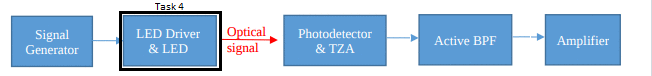
\includegraphics[width=.9\textwidth ]{Introduction/Block_Diagram_MFBP.png}
    \caption{Block diagram for optical uplink \cite{b1}}
    \label{fig:blockdiagram2}
\end{figure}

The voltage amplifier is required by the optical uplink project. The output signal from the multi-feedback bandpass filter (MFBP) is in the hundreds of millivolt range. In order to make a more easily detectable signal, a voltage amplifier is required. This can achieved through the use of either a common source or common emitter amplifier. The specifications for this lab are summarized in Table \ref{tab:specifications}.

\begin{table}[H]
	\centering
	\caption{Voltage amplifier specifications}
	\label{tab:specifications}
	\begin{tabular}{|l|l|}
		\hline
		Specifications & Required       \\ \hline
		Peak gain, with load      & 21 dB $\pm$ 1dB\% \\ \hline
		Bias current for N$_1$     & ~1mA          \\ \hline
		Lower cut-off frequency      & $\geq$100 mA    \\ \hline
		Upper cut-off frequency    &  at least 200 kHz \\ \hline
		R$_{in}$, small signal       &  at least 1 M$\Omega$ \\ \hline
		R$_{out}$, small signal      &  at least 3 k$\Omega$ \\ \hline
		2$^{nd}$ Harmonic distortion $@$ 1kHz  & $<$2\% \\ \hline
		Supply voltages            &  $\pm$12 V     \\  \hline
	\end{tabular}
\end{table}


The voltage amplifier circuit receives the voltage signal from the MFBP and increases the amplitude of the voltage wavefrom. The desired final output being 5 V. This is achieved with either the use of a NMOS common source amplifier or an NPN BJT common emitter amplifier.


Section 2 of this report describes the design and simulations of the common source amplifier and the common emitter amplifier. Experimental results are addressed in section 3. A discussion of the results, sources of error, and areas of possible improvement are outlined in section 4. Section 5 concludes this report. \newline



\end{document}